\section{Introduction}
The range of bacterial growth rates is enormously diverse. In natural
environments, some microbial organisms might double only once per year while
in comfortable laboratory conditions, growth can be rapid with several
divisions per hour. This six order of magnitude difference illustrates the
intimate relationship between environmental conditions and the rates at which
cells convert nutrients into new cellular material -- a relationship that has
remained a major topic of inquiry in bacterial physiology for over a century
\citep{jun2018}. As was noted by Jacques Monod, ``the study of the growth of
bacterial cultures does not constitute a specialized subject or branch of
research, it is the basic method of Microbiology.’’ Those words ring as true
today as they did when they were written 70 years ago. Indeed, the study of
bacterial growth has undergone a molecular resurgence since many of the key
questions addressed by the pioneering efforts in the middle of the last
century can be revisited by examining them through the lens of the
increasingly refined molecular census that is available for bacteria such as
the microbial workhorse \textit{Escherichia coli}. Several of the outstanding
questions that can now be studied about bacterial growth include: what sets
the fastest time scale that bacteria can divide, and how is growth rate tied
to the quality of the carbon source. In this paper, we address these two
questions from two distinct angles. First, as a result of an array of
high-quality proteome-wide measurements of the \textit{E. coli} proteome
under a myriad of different growth conditions, we have a census that allows
us to explore how the number of key molecular players change as a function of
growth rate. This census provides a window onto whether the processes they
mediate such as molecular transport into the cells and molecular synthesis
within cells can run faster. Second, because of our understanding of the
molecular pathways responsible for many of the steps in bacterial growth, we
can also make order of magnitude estimates to infer the copy numbers that
would be needed to achieve a given growth rate. In this paper, we pass back
and forth between the analysis of a variety of different proteomic datasets
and order-of-magnitude estimations to determine possible molecular
bottlenecks that limit bacterial growth and to see how the growth rate varies
in different carbon sources.

Specifically, we leverage a combination of \textit{E. coli} proteomic data
sets collected over the past decade using either mass spectrometry
\citep{schmidt2016,peebo2015, valgepea2013} or ribosomal profiling
\citep{li2014} across 31 unique growth conditions. Broadly speaking, we
entertain several classes of hypotheses as are illustrated in
\FIG{categories}. First, we consider potential limits on the transport of
nutrients into the cell. We address this hypothesis by performing an
order-of-magnitude estimate for how many carbon, phosphorous, and sulfur
atoms are needed to facilitate this requirement given a 5000 second division
time. As a second hypothesis, we consider the possibility that there exists a
fundamental limit on how quickly the cell can generate ATP. We approach this
hypothesis from two angles, considering how many ATP synthase complexes must
be needed to churn out enough ATP to power protein translation followed by an
estimation of how many electron transport complexes must be present to
maintain the proton motive force. A third class of estimates considers the
need to maintain the size and shape of the cell through the construction of
new lipids for the cell membranes as well as the glycan polymers which make
up the rigid peptidoglycan. Our final class of hypotheses centers on the
synthesis of a variety of biomolecules. Our focus is primarily on the stages
of the central dogma as we estimate the number of protein complexes needed
for DNA replication, transcription, and protein translation.

In broad terms, we find that the majority of these estimates are in close
agreement with the experimental observations, with protein copy numbers
apparently well-tuned for the task of cell doubling. This allows us to
systematically scratch off the hypotheses diagrammed in \FIG{categories} as
setting potential growth bottlenecks. Ultimately, we find that protein
translation (particularly the generation of new ribosomes) acts as 1) a rate
limiting step for the \textit{fastest} bacterial division, and 2) a major
determinant of bacterial growth across the nutrient conditions we have
considered under steady state, exponential growth. This perspective is
consistent with the linear correlation observed between growth rate and
ribosomal content (typically quantified through the ratio of RNA to protein) for
fast growing cells \citep{scott2010}, but also suggest a more prominent role for
ribosomes in governing the changes in cell size and doubling time across all
conditions of nutrient limitation.

% Here we
% again leverage the quantitative nature of this data set and present a
% quantitative model of the relationship between the fraction of the proteome
% devoted to ribosomes and the speed limit of translation, revealing a fundamental
% tradeoff between the translation capacity of the ribosome pool and the maximal
% growth rate.

% with single-cell and single-protein resolution using modern methods of video
% microscopy \citep{si2017,harris2018} and through advances in mass spectrometry and
% sequencing technologies \citep{schmidt2016,li2014}. This has permitted
% quantitative insight into how bacteria like \textit{E. coli} allocate their
% cellular resources under nutrient-limitation, and following genomic and
% pharmacological perturbations \citep{scott2010,hui2015,basan2015}.
% This body of experimental data places us in the auspicious position to
% explore how the abundance of essential protein complexes are related to the
% growth rate of the population and interrogate what biological processes may set
% the speed limit of bacterial growth.

% In this work, we seek to leverage a collection of proteomic data sets of
% \textit{Escherichia coli} across 31 growth conditions \citep{valgepea2013,li2014,
% peebo2015,hui2015,schmidt2016} to quantitatively explore what biological
% processes may set the speed limit of bacterial growth.

% Might be important to acknowledge, like done in Scott2010
% that this is the expectation noted long ago by mass-balance considerations,
% in O. Maaløe, in Biological Regulation and Development,
% R. F. Goldberger, Ed. (Plenum, New York, 1979),
% pp. 487–542'

\begin{figure}
    \centering{
    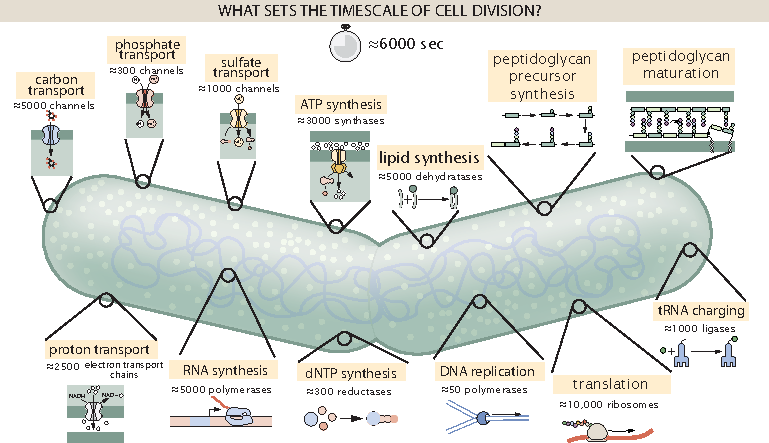
\includegraphics{main_figs/schematic_categories.pdf}
    \caption{\textbf{Transport and synthesis processes necessary for cell division.}
            We consider an array of processes necessary for a cell to double its
            molecular components. Such processes include the transport of carbon
            across the cell membrane, the production of ATP, and fundamental
            processes of the central dogma namely RNA, DNA, and protein
            synthesis. A schematic of each synthetic or transport category is
            shown with an approximate measure of the complex abundance at a
            growth rate of 0.5 per hour. In this work, we consider a standard bacterial division time of
            $\approx$ 5000 sec.}
    \label{fig:categories}
    }
\end{figure}
